\chapter{Introduction}
\label{ch:intro}

\section{Problem Statement}
The state of Alaska currently has dozens of communities which are electrically isolated from the rest of the state. They effectively act as remote permanently islanded microgrids. These communities typically use diesel generators to provide most of their electrical power. Power sources such as coal or natural gas are less expensive in larger grids but these microgrids are too small to take advantage of such economies of scale. This makes it expensive to operate relative to the size of the communities. Furthermore, the remoteness of these communities significantly increases the cost to import fuel.

The goal of this thesis is to determine an affordable method to incorporate renewable energy into microgrids without compromising stability and reliability. One method of reducing operating costs is to offset diesel fuel through the use of locally available renewable energy resources.\footnote{Sometimes called renewables, these sources of energy either will not be depleted or can be replenished in a reasonably short period of time. They include wind, sunlight, geothermal heat, biomass, and water flow.} Unfortunately powering a microgrid with a significant portion of intermittent renewable resources can negatively impact grid stability unless appropriate infrastructure is included. 

This thesis will seek to accomplish its goal by simulating the operation of a permanently islanded microgrid containing geothermal power generation under multiple scenarios and cases. 
\begin{itemize}
\item One greenfield site will be examined with no existing permanent electrical infrastructure.
\item One brownfield site will be examined where there is an existing grid connection but experiences regular outages.
\item In both cases the geothermal power will be converted from AC to DC then back to AC in to be distributed to the loads.  
\end{itemize}

The greenfield area selected for the microgrid, Pilgrim Hot Springs, lies about 60 miles north of Nome in western Alaska. Since the 1970s there has been interest in developing the hot springs in order to generate electricity similar to the organic Rankine cycle generator used in Chena Hot Springs. Several exploratory wells have been drilled and indicate potential for low temperature geothermal electrical generation \cite{Holdmann2013}. \autoref{fig:pilgrimFLIR} shows a geothermal runoff stream and how much warmer the water is compared to the banks. The area is currently undeveloped,\footnote{There are historic ruins of an old church and orphanage from the early 1900s, but those buildings are uninhabitable.} therefore this remote microgrid will be designed from scratch. The land owners, Unataaq LLC, have expressed interest in developing the resource as a tourist attraction, for agriculture, as well as for electrical production.
\begin{figure}[hb]
	\centering
	
	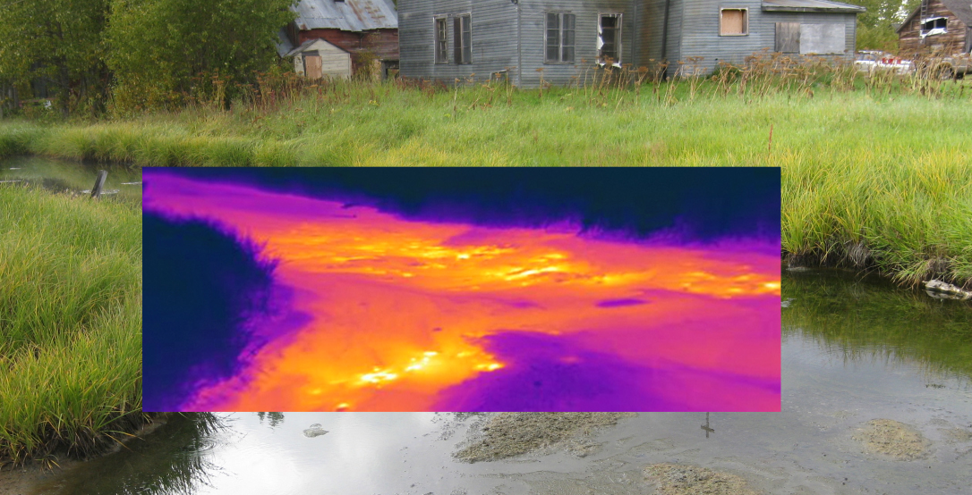
\includegraphics[width=\textwidth]{figures/PilgrimFLIR.png} 

	\caption{A FLIR thermal camera image of a Pilgrim Hot Springs geothermal runoff stream overlayed onto a photo. Credit: ACEP}
	\label{fig:pilgrimFLIR}


\end{figure}

Iceland has extensive experience utilizing their geothermal resources, but so far only high temperature areas are used for electricity production, while low temperature sites are used for district heating. One such system, an the brownfield case study, heats the community of Bergsta$\eth$ir, Iceland, a rural area in the northern part of the island. \autoref{fig:bergstadir_effluent} shows the discharge pipe and steaming effluent of the system. The pumps used to circulate the water are electrically driven by two \SI{15}{\kilo\watt} motors, but electrical grid in rural Iceland is less reliable than the heating loop needs to be. Currently the community uses diesel generators to power the pumps when the electricity goes out, but they are interested in alternatives.
\begin{figure}[h]
	\centering
	\caption{District heating effluent at Bergssta$\eth$ir, Iceland. Credit: George Roe.}
	\label{fig:bergstadir_effluent}
	
	
\includegraphics[width=\textwidth]{figures/BergstadirEffluent.jpg} 


\end{figure}

\section{Microgrid Description}
Microgrids are electrical systems composed of sources and loads within a well defined electrical boundary. Many microgrids are connected to a larger grid but with the ability to become separated, or islanded, while still maintaining some or all of the loads. Others need to remain connected but still maintain a boundary. Some form of energy storage is often used for systems operating independently from the larger grid. This section will describe the key components and characteristics of a microgrid with emphasis on relevance to Alaska.

Approximately 70\% of the population of Alaska is connected to a single grid called the Railbelt \cite{railbelt}. The Railbelt stretches over 600 miles from the Homer on the Kenai Peninsula to the greater Fairbanks area in the interior and includes most communities on the road system in between. The remaining communities and villages can be considered permanently islanded microgrids. Each has loads that need power, some power source, some system of storing the energy or fuel.

A microgrid can operate using Alternating Current (AC), Direct Current (DC), or a hybridization of the two. The choice to whether to use AC\footnote{Unless otherwise noted, AC will refer to three phases separated by a phase angle of 120\textdegree{} rather than a single phase.} or DC depends on the demand of the loads, the available power sources and conversion devices, as well as the existing electrical infrastructure. The decision between AC and DC goes as far back as 1880s when George Westinghouse and Thomas Edison were competing to supply America with electrical power. Ultimately Westinghouse and AC came out on top in part due to its relative ease of transforming to high voltage and low current which transmits more efficiently. Furthermore, electric machinery that use AC to generate rotating magnetic fields operate more efficiently than machines which use DC power and commutators. More recently however, computers and other electronic devices which use DC have become much more prolific, which has led to a renewed call for DC systems. Like most of the world, Alaska uses AC networks and converts to DC as necessary at the device level.

\subsection{Loads}
Well designed microgrids are configured around expected loads. Loads can require active as well as reactive power. Reactive power cannot do any net work, but is generally used to maintain magnetic or electric fields in inductive loads. Any work done by the field, such as a magnetic field spinning a rotor, is due to active power. Active power, also called real power, is associated with resistive loads. While resistive loads consume active power and inductive loads consume reactive power, capacitive loads generate reactive power and are often used to reduce the reactive power supplied by the sources. 

Regardless of the type of load, there must always be a power balance among sources, loads, storage, and losses. If the total load increases too high, either additional sources must be brought online or other loads must be shed. It costs money to bring more sources online, particularly fuel based sources, therefore it is better to decrease the load if possible. Certain flexible loads can be designated as dispatchable. They require a certain amount of energy over a period of time but not continuously or on demand. These loads can be shut off automatically or forced to remain off during periods of high energy use. Additionally if the power generated by intermittent renewable resources exceeds the power consumed by normal loads, dispatchable loads can be activated sooner than they otherwise would be. This can potentially maximized fuel displacement of the renewable resource. However, the dispatchable loads require additional infrastructure and controls in order to communicate with other grid components to know when it is appropriate to turn on and off.

\subsection{Sources}
Microgrid power is typically generated by Distributed Energy Resources (DER). This can include renewable resources such as solar photovoltaics, wind turbine generators, and geothermal generators as well as and non\--re\-new\-able sources such diesel generators and natural gas micro-turbines. 
%Most power sources generate AC power. Current is induced by rotating coils withing a magnetic field

Diesel generators use the combustion of diesel fuel to spin an alternator producing AC power. These generators are prolific in rural Alaska generally being used as the prime mover to regulate grid frequency and voltage. The communities  generally purchase the fuel in bulk once or twice each year because of their remote locations. The fuel is then stored in tank farms until used.
%These generators are composed of an engine, alternator, fuel system, excitation system, governor, cooling system, exhaust system, and turbocharger.
Due to the widespread use of diesel generators in Alaska, significant energy cost savings can be generated by reducing fuel consumption through efficiency improvements and use of alternate energy sources. 

Geothermal generators are heat engines and can operate similarly to traditional coal and nuclear plants. Heat causes a working fluid to thermally expand and change phases thus spinning a turbine to produce AC power. The primary difference is that geothermal systems get heat from the Earth as opposed to combustion or nuclear reactions. Geothermal generators can be divided into high heat and low heat categories. High heat geothermal systems work with temperatures well above the boiling point of water which means water can be used as the working fluid. Low heat systems operate at temperatures near or below the boiling point of water therefore a refrigerant must be used as an alternative working fluid. 
%talk about chena hotspings as an example of existing geothermal in AK

%Wind turbine generators produce what is known as wild AC, where frequency and voltage are unregulated and can vary with wind speed. Modern wind turbines have built-in methods of ensuring the generated power is usable by the grid.
%\begin{verbatim} 
% address gearboxes  
% various wind turbine conversion topologies perhaps
% talk about wind resources of western alaska
%\end{verbatim}

%Solar photovoltaic (PV) panels generate DC power. Panels are made up of a string of cells of a semiconductor material. The most commonly used material is Silicon, but Gallium Arsenide (GaAr), Cadmium Telluride (CdTe), and Copper Indium Gallium Selenide (CIGS) can be used in certain applications as well. Regardless of the material, all PV panels operate by absorbing sunlight and exciting electrons to higher energy orbital. Some fraction of the excited electrons become free and capable of generating a current. PV systems in Alaska face certain challenges due to the long dark winters, however there are also several beneficial characteristics. Solar PV cell operate more efficiently in colder temperatures and reflection due to high albedo of snow can increase the light incident on appropriately positioned panels. During the months of March and April, twelve or more hours of sunlight are available, but temperatures remain relatively cool and the ground remains covered in snow. For those reasons solar PV can be especially competitive in the Alaskan spring.

\subsection{Storage}
Energy storage is beneficial to microgrid operation because it allows generation to be spread over time. Energy Storage Systems (ESS) can include batteries, flywheels, super-capacitors, pumped hydro, and more. These devices have different storage duration and discharge times making various storage technologies advantageous in different situations \cite{Schoenung2003}. The discharge of bulk energy storage over the course of many hours allows for load leveling and provides spinning reserve for the grid.\footnote{Spinning reserve is extra operating capacity capable of responding to sudden load increases at will.} Load peak shaving typically involves a discharge time from minutes to several hours. Energy storage discharge over seconds and sub-seconds is generally done to improve power quality.

%Bulk diesel fuel tanks can provide an alternative method of energy storage.

\subsection{Conversion}
Electronic conversion devices take a form of electrical power (AC or DC) and convert it into a different form. Power conversion devices typically use switching components such as diodes or transistors to control the general wave form of the output.\footnote{The major exceptions are transformers.} Inductors and capacitors provide filtering as well as ensure continuous levels of the voltage and current waveforms. Inverters convert DC power into sinusoidal AC power. Rectifiers convert AC to DC. DC-DC converters can step up or down the voltage level of a DC power source. Transformers can step up or down the voltage level of an AC source while maintaining frequency by magnetic induction. Variable Frequency Drives (VFD)\footnote{Sometimes called Variable Speed Drives (VSD)} modify the frequency of an AC source, and typically involves rectifying the source then inverting then that output at the desired frequency. 
%address high frequency transformers: isolation + additional voltage step up/down
%maybe in conversion chapter



%\paragraph{}
%More advanced methods and architectures of power conversion will be addressed further in \autoref{ch:conv}.

\subsection{Control}
A microgrid control system ties all the other components together. Control systems monitor and maintain the voltage and frequency of the grid while ensuring sufficient active and reactive power is supplied to the loads. The control schemes of power sources and converters can generally be divided into several categories: grid forming, grid following, grid supporting, and grid parallel \cite{Ortjohann2012, Engler, Strauss2003}. 

Grid forming units set the frequency and voltage levels of the microgrid. Grid following units control the power\footnote{Both active power and reactive power.} supplied to the grid based on external reference values from the loads. As loads demand more power, a grid following unit will supply more power within is capabilities. Grid supporting units provide power based on voltage and frequency regulation. They assist the grid forming unit with maintaining the voltage and frequency while also supplying power. Grid parallel units also supply power to the grid, but it is based on reference values of a source. These units typically incorporate a Maximum Power Point Tracking (MPPT) algorithm in order to produce as much power as is available. They are used with intermittent sources such as wind turbines and solar PV arrays. 

Control over DER and conversion units can also be categorized by whether or not communication is used. Typically communication among units can yield more precise power sharing and set points but the necessary communication lines can introduce additional costs and points of failure \cite{Vandoorn2013}. Furthermore, control strategies that do not require communication are easier to expanded and provide redundancy because coordination among controller units is less complex. Methods of communication based control includes centralized control, distributed control, Master\slash Slave control, etc. Methods of non-communication based control includes droop control as well as frequency based signal injection.

\subsubsection{Communication Based Control}
Centralized control schemes make use of two way communication where a central controller sets the priorities of local DER and load controllers during regular intervals. The priorities are determined from a predefined optimization algorithm and uses inputs of the supply and demand from the local controllers, as well as market costs during the previous interval \cite{Katiraei2008}. Distributed control schemes also use a centralized control unit to regulate the set points of the local control units, but simpler communications are used. The central control unit responds more slowly to disturbances than the local controllers, but helps ensure they share power evenly in steady state conditions \cite{Prodanovic2006}. 

In a master\slash slave relationship between different DER units, the master will operate in voltage control mode and the slave units in current control mode. Such a system may or may not include a central controller. Without a central controller, the master sets the current reference for the remaining units \cite{Siri1992}. If there is a central controller then it is the controller, not the master that sets the current references \cite{Chen1995}.

\subsubsection{Non-Communication Based Control}
\label{sec:droop}
The droop control method originated with the relationship between frequency and active power for synchronous machines due to rotating inertia. As a load increases the machine will slow and its frequency will droop. It has since been adapted into power conversion control schemes as well despite the lack of physical inertia. It is mathematically derived from the equation describing active power flow through an impedance $ R + jX $ from point 1 to point 2.
\begin{equation}
P = \frac{V_{1}}{R^2 + X^2} \big( R \left( V_{1}-V_{2}\cos{\delta_{12}} \right) +X V_{2} \sin{\delta_{12}} \big)
\end{equation}
Assuming small phase angle $\delta_{12}$ between the points as well as negligible resistance $R$, the equation can be reduced to 
\begin{equation}
P = \frac{V_1V_2}{X}\delta_{12}
\end{equation}
In practice, the frequency is used rather than the angle because individual units do not know the phase of other units due to the lack of communication. For power and frequency deviation from predefined references the droop equation becomes
\begin{equation}
f = f_{\text{ref}} + K_P\left(P - P_{\text{ref}}\right)
\end{equation}
where $K_P$ is a negative proportionality constant.

Similarly a droop relationship between reactive power flow and relative voltage levels can be shown:
\begin{equation}
Q = \frac{V_1}{R^2 + X^2} \big( -R V_2 \sin{\delta_{12}} + X \left(V_1 - V_2 \cos{\delta_{12}}\right) \big)
\end{equation}
\begin{equation}
Q = \frac{V_1}{X} \left( V_1 - V_2 \right)
\end{equation}
\begin{equation}
V = V_{\text{ref}} + K_Q \left( Q - Q_{\text{ref}} \right)
\end{equation}
where $K_Q$ is a negative proportionality constant. 

It should be noted, however, the droop equations are only valid under certain conditions. If the angle/frequency deviations are too great then the small angle approximations will break down. Additionally, the relative magnitude of the resistive and reactive impedance components effect system dynamics. If the frequency changes are too great then $X$ can no longer be considered constant. This means the $P$\slash $f$ and $V$\slash $Q$ relationships cannot be approximated as linear. Additionally, the line resistance in most low voltage systems is not so small as to be negligible. In fact in situations where the line reactance is negligible compared to the resistance, then linear approximations can be made between active power and voltage as well as reactive power and frequency \cite{YunWeiLi2009}.


%distributed control vs centralized
%droop control vs Master/slave
%Katiraei et al & Vandoorn et al

\section{AC vs DC Microgrids}
AC microgrids and DC microgrids are both technically feasible, but the selection of which is optimal heavily depends on the types of loads and power sources used. Furthermore, the choice is not necessarily a binary decision. AC\slash DC hybrid systems can provide benefits of each, but at greater cost. This section will compare and contrast the different architectures.

\subsection{Efficiency}
In each conversion step there is some power loss due to inefficiencies. Sequential conversions can add up to a significant losses. Distributing AC and DC power to their respective loads separately can eliminate many conversion steps but it is unrealistic to completely remove all steps. \autoref{tab:conv_eff} shows that, at rated values, typical losses among different power converters are not symmetric. Transformers are the most efficient, followed by inverters and DC-DC converters. Rectifiers are experience the most loss. When operated below rated values all conversion devices experience drops in efficiency.

\begin{table}[]
\centering
\caption{Efficiencies of typical power conversion devices.}
%Keep an eye out for efficiency values more recent the 2006 and 2008
\label{tab:conv_eff}
\begin{tabular}{|ll|l|l|}
\hline
	&				& \multicolumn{1}{l}{From}	&				\\ \cline{3-4} 
	&				& AC				& DC				\\ \hline 
To	& \multicolumn{1}{|l|}{AC}	& 98\% \cite{Starke2008}	& 90\% \cite{Pang2006}	\\ \cline{2-4} 
	& \multicolumn{1}{|l|}{DC}	& 97\% \cite{Starke2008}	& 95\% \cite{Starke2008}	\\ \hline
\end{tabular}
\end{table}
 
% Keep a look out for conversion efficiency more recent than 2006 and 2008

Additionally, distribution power losses are not identical for AC and DC systems. For an AC and DC\footnote{Assuming a DC neutral line introduced.} system, each delivering the same active power and experiencing equal distribution losses, the relationship of RMS current is given as $\frac{I_{AC}}{I_{DC}} = \sqrt{\frac{2}{3}} \approx 0.82$ and a RMS voltage relationship is $\frac{V_{AC}}{2V_{DC}} = \frac{1}{\cos{\theta}} \sqrt{\frac{2}{3}} \approx \frac{0.82}{\cos{\theta}}$ where $\theta$ is the phase angle between $V_{AC}$ and $I_{AC}$ \cite{Starke2008}. Despite the small advantage of DC has over AC in this respect, distribution losses in are typically smaller than losses due to conversion.

\subsection{Stability}
Electric machinery and power electronic conversion devices introduce undesired harmonics into AC grids due to non-linear loading effects \cite{Grotzbach1997}. Harmonic distortion can cause power losses as well as reduce voltage and frequency stability. Because harmonics are, by definition, based off of a fundamental frequency the harmonics alone are not an issue in DC segments of a microgrid system. DC systems can experience stability issues caused by non-linear loads such as spikes in current and voltage.

Another important factor in grid stability is how quickly and safely the system can clear an electrical fault. The sinusoidal oscillation of AC systems means there is a periodic zero crossing 60 times each second.\footnote{For regions that operate on 60 Hz.} This means faults can be cleared more quickly in AC systems than in DC systems.  However, AC systems typically experience larger transient spikes during fault events when compared to comparable DC systems \cite{Estes2011}. 

\subsection{Economics}
Most existing electrical infrastructure is built around AC grids rather than DC grids. Furthermore off the shelf electrical appliances generally assume AC power is available and will rectify to DC if needed. These factors indicate the installation of an AC distribution system is more economical. However, AC systems require three lines for each phase, and sometimes a forth neutral line, while DC systems only require two, and sometimes a third neutral line.\footnote{Although work has been done on Single Line Ground Return systems which only require one line.} Although the economic benefit of fewer electrical lines is much more significant to long distance transmission rather than distribution to near by loads.

One benefit of DC microgrids over AC is the necessity to control only voltage level rather than voltage and frequency. A simplified control scheme can reduce the cost combining power sources into a DC bus before distribution avoids the necessity of synchronization \cite{Lotfi2015}.

\section{Thesis Organization}
With the background information on microgrids addressed in \autoref{ch:intro} above, the remainder of the thesis will be organized as followed: \autoref{ch:conv} will delve deeper into background of power conversion. This includes the conversion of heat to electricity, with a focus on low-temperature sources, as well electrical power conversion, focusing on the pros and cons of different topologies. 
%\autoref{ch:geothermal} will address necessary background on geothermal power generation. 
\autoref{ch:model} will detail the model and its validation. \autoref{ch:analysis} will analyze the simulation results of the greenfield and brownfield scenario.  \autoref{ch:conclusion} will conclude the thesis and describe future work to be conducted on the topic.

